L'exercice est constitué de deux parties indépendantes.


\medskip

\noindent {\Large \textbf{Partie 1}}

\medskip

Pour tout entier $n$ supérieur ou égal à 1, on désigne par $f_{n}$ la fonction définie sur $[0~;~1]$ par :
\[f_{n}(x) = x^{n} \e^{x}\]

On note $C_{n}$ la courbe représentative de la fonction $f_{n}$ dans un repère \Oij{} du plan.

On désigne par $\left(I_{n}\right)$ la suite définie pour tout entier $n$ supérieur ou égal à 1 par :
\[I_{n} = \int_{0}^{1} x^{n} \e^{x} \mathrm{~d} x.\]

\begin{enumerate}
\item 
	\begin{enumerate}
		\item On désigne par $F_{1}$ la fonction définie sur $[0 ; 1]$ par :
\[F_{1}(x) = (x-1) \e^{x}.\]

Vérifier que $F_{1}$ est une primitive de la fonction $f_{1}$.

		\item Calculer $I_{1}$.
	\end{enumerate}
\item À l'aide d'une intégration par parties, établir la relation pour tout $n$ supérieur ou égal à 1 ,
\[I_{n + 1} = \e-(n + 1) I_{n}.\]

\item Calculer $I_{2}$.

\item On considère la fonction \texttt{mystere} écrite dans le langage Python :

\begin{center}
	\renewcommand\arraystretch{1}
	\texttt{\begin{tabular}{l}
			from math import e \# la constante d'Euler e \\
			\\
			def mystere(n):\\
			\quad a = 1\\
			\quad L = [a]\\
			\quad for i in range(1,n):\\
			\quad\quad a = e - (i + 1)*a\\
			\quad\quad L.append(a)\\
			\quad return L\\
	\end{tabular}}
	\renewcommand\arraystretch{1.4}
\end{center}

À l'aide des questions précédentes, expliquer ce que renvoie l'appel \texttt{mystere(5)}.
\end{enumerate}


\medskip

\noindent {\Large \textbf{Partie 2}}

\medskip


\begin{enumerate}
	\item Sur le graphique ci-dessous, on a représenté les courbes $C_{1}, C_{2}, C_{3}, C_{10}, C_{20}$ et $C_{30}$.

\medskip

\hspace*{-1.5cm}	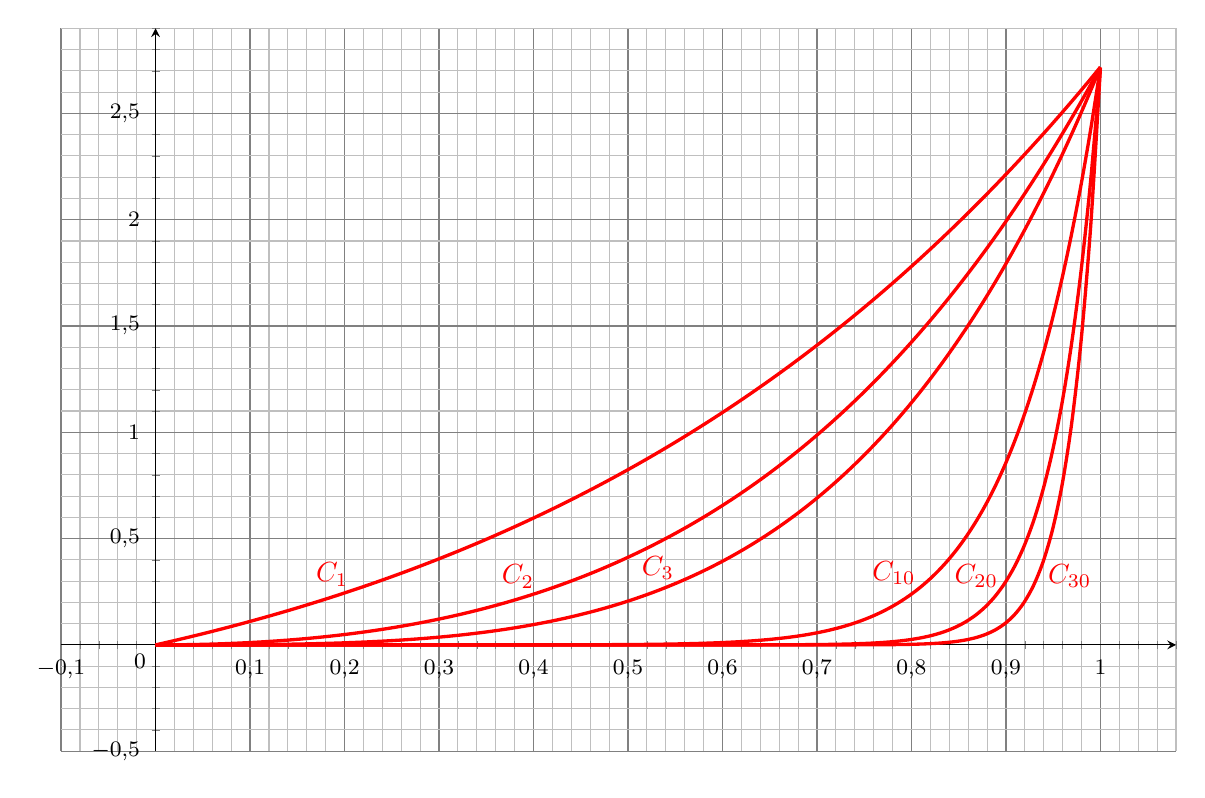
\begin{tikzpicture}
				\begin{axis}[/pgf/number format/use comma,x = {120mm},y = {27mm}, xmin = -0.1, xmax = 1.08, ymin = -0.5, ymax = 2.9, xtick distance = 0.1, ytick distance = 0.5,
					tick label style = {font = \footnotesize},
					 minor tick num = 4, grid = both, major grid style = {line width = .5pt,draw = gray}, axis lines = center]
					\addplot [line width = 1.2pt, color = red, smooth, samples = 100, domain = 0:1 ]{x*exp(x)} node[pos = 0.1,above] {$C_1$};
					\addplot [line width = 1.2pt, color = red, smooth, samples = 100, domain = 0:1 ]{x^2*exp(x)} node[pos = 0.15,above] {$C_2$};
					\addplot [line width = 1.2pt, color = red, smooth, samples = 100, domain = 0:1 ]{x^3*exp(x)} node[pos = 0.2,above] {$C_3$};
					\addplot [line width = 1.2pt, color = red, smooth, samples = 100, domain = 0:1 ]{x^(10)*exp(x)} node[pos = 0.3,left] {$C_{10}~$};
					\addplot [line width = 1.2pt, color = red, smooth, samples = 100, domain = 0:1 ]{x^(20)*exp(x)} node[pos = 0.32,left] {$C_{20}$};
					\addplot [line width = 1.2pt, color = red, smooth, samples = 100, domain = 0:1 ]{x^(30)*exp(x)} node[pos = 0.33,right] {$C_{30}$};
					\node[below left] at (axis cs: 0,0) {{\footnotesize 0}};
				\end{axis}
			\end{tikzpicture}

	\begin{enumerate}
		\item Donner une interprétation graphique de $I_{n}$.

		\item Quelle conjecture peut-on émettre sur la limite de la suite $\left(I_{n}\right)$ ?
	\end{enumerate}
\item Montrer que pour tout $n$ supérieur ou égal à 1,
\[0 \leqslant I_{n} \leqslant \e \int_{0}^{1} x^{n} \mathrm{~d} x.\]
		\item En déduire $\lim\limits_{n \to + \infty} I_{n}$.
	\end{enumerate}
